\documentclass[12pt]{article}
\usepackage[english]{babel}
% \usepackage[utf8x]{inputenc}
\usepackage[T1]{fontenc}
\usepackage{scribe}
\usepackage{listings}
\usepackage{fullpage}
\usepackage{amsfonts}
\usepackage{amssymb}
\usepackage{hyperref}
\usepackage{url}
\usepackage[svgnames]{xcolor}
\usepackage{color}
\usepackage{subcaption}
\usepackage{booktabs}
\usepackage{multicol}
% \definecolor{light-gray}{gray}{0.90}
% \lstset{backgroundcolor=\color{light-gray},showlines=true}

% \usepackage{xcolor}
% \usepackage{listings}

% \lstdefinestyle{BashInputStyle}{
%   language=bash,
%   basicstyle=\small\sffamily,
%   numbers=left,
%   numberstyle=\tiny,
%   numbersep=3pt,
%   frame=tb,
%   columns=fullflexible,
%   backgroundcolor=\color{yellow!20},
%   linewidth=0.9\linewidth,
%   xleftmargin=0.1\linewidth
% }

\usepackage{minted}
\setminted{fontsize=\footnotesize,baselinestretch=0.5}

\Scribe{}
\Lecturer{Queenie Qiu, John Raiti. Student: \textbf{Shucheng Guo}}
\LectureNumber{5}
\LectureDate{DATE: Feb 16th. 2023}
\LectureTitle{Introduction to Robotic Arm Kinematics}

\lstset{style=mystyle}

\begin{document}
	\MakeScribeTop

%#############################################################
%#############################################################
%#############################################################
%#############################################################

\section{Learning Objectives}
\begin{enumerate}
    \item Learn the difference between arm motions in task-space and configuration-space.
    
    \item Familiarize yourself with MoveIt! as a ROS component.
    
    \item Implement high-level nodes through MoveIt! combined with RViz and Gazebo to move a Kinova Gen3lite arm and a Fetch robotics arm using forward and inverse kinematics.
\end{enumerate}


\section{Introducing Kinova Gen3lite
}
\subsection{ROS Kortex Package Installation}
ROS Kortex is the official ROS package to interact with Kortex and its related products. These are the instructions to run in a terminal to clone the ros\_kortex repository and install the necessary ROS dependencies. \\
\textbf{Note}:The default branch for git clone is developed for ROS Noetic. If you are using other ROS distributions, please git clone to corresponding branch.
\begin{minted}{bash}
    $ sudo apt install python3 python3-pip
    $ sudo python3 -m pip install conan
    $ conan config set general.revisions_enabled=1
    $ conan profile new default --detect > /dev/null
    $ conan profile update settings.compiler.libcxx=libstdc++11 default
    $ cd catkin_ws/src
    $ git clone https://github.com/Kinovarobotics/ros_kortex.git
    $ cd ../
    $ rosdep install --from-paths src --ignore-src -y
    \end{minted}
Then, to build and source the workspace:
\begin{minted}{bash}
    $ catkin_make
    $ source devel/setup.bash
    \end{minted}

\subsection{Spawning a Kinova Gen3lite robot in Gazebo}

We will use the ros\_kortex repository to work with the Kinova arm. In this metapackage, we will use the kortex\_gazebo portion for simulation. Execute the following launch file that will bring up a gen3lite in Gazebo and open an RViZ window
\begin{minted}{bash}
    $ roslaunch kortex_gazebo spawn_kortex_robot.launch arm:=gen3_lite z0:=0.0
    \end{minted}

The Gazebo window looks like:

\begin{figure}[H]
    \vspace{-10pt}
    \centering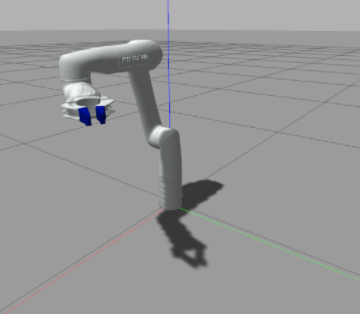
\includegraphics[width=5cm]{images/gazebo.PNG}\vspace{-10pt}
    \caption{Spawning in Gazebo.}\label{fig:gazebo}
    \end{figure}

Note: Once the RViZ and Gazebo windows have been opened, and the terminal shows two green messages ( “You can start planning now!” and “The Kortex driver has been initialized correctly!” ) you can add a Robot model and add a MotionPlanning component in Rviz.

\begin{figure}[H]
    \vspace{-10pt}
    \centering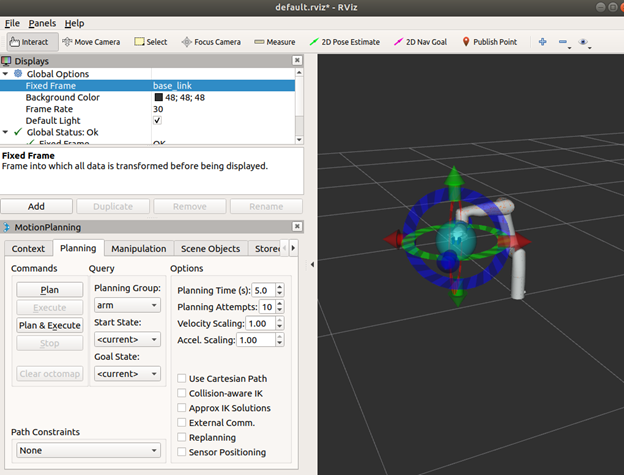
\includegraphics[width=10cm]{images/rviz1.png}\vspace{-10pt}
    \caption{Kinova arm in Rviz.}\label{fig:rviz1}
    \end{figure}

\subsection{Using the Interactive Markers to change the robot’s pose based on the task-space}


You can use the different arrows and rings on the interactive marker, to change positions and orientations of the robot’s end-effector. As you use them, you will see an orange version of the robot arm with the proposed new position. Once you have reached a desired position, use the buttons “Plan” and “Execute”(in the MotionPlanning Panel) to make the robot in Gazebo move to the new proposed position. Some useful tools for you to track the robot’s motions are:

\begin{enumerate}
    \item Check the values of the joints:
        \begin{minted}{bash}
        $ rostopic echo -n 1 /my_gen3_lite/joint_states
        \end{minted}
    \item Outputs the pose of the robot’s end-effector with respect to the world (in this case Gazebo’s origin):

        \begin{minted}{bash}
        $ rosrun tf tf_echo /world /end_effector_link
        \end{minted}

    \item You may also consider using the base link as the reference:
        \begin{minted}{bash}
        $ rosrun tf tf_echo /base_link <END-EFFECTOR LINK>
        \end{minted}
\end{enumerate}    
If you want to change the state of the gripper, you need to change the Planning Group (in the MotionPlanning Panel) from arm to gripper, and you can select a new position.\\

\textbf{Deliverables:}
\begin{enumerate}
    \item Add a TF component in RViz and enable only the base\_link and the end\_effector\_link. Disable the Motion Planning component to temporarily remove the interactive markers. Add a screenshot of the RViZ view.
    
    \begin{figure}[h]
        \centering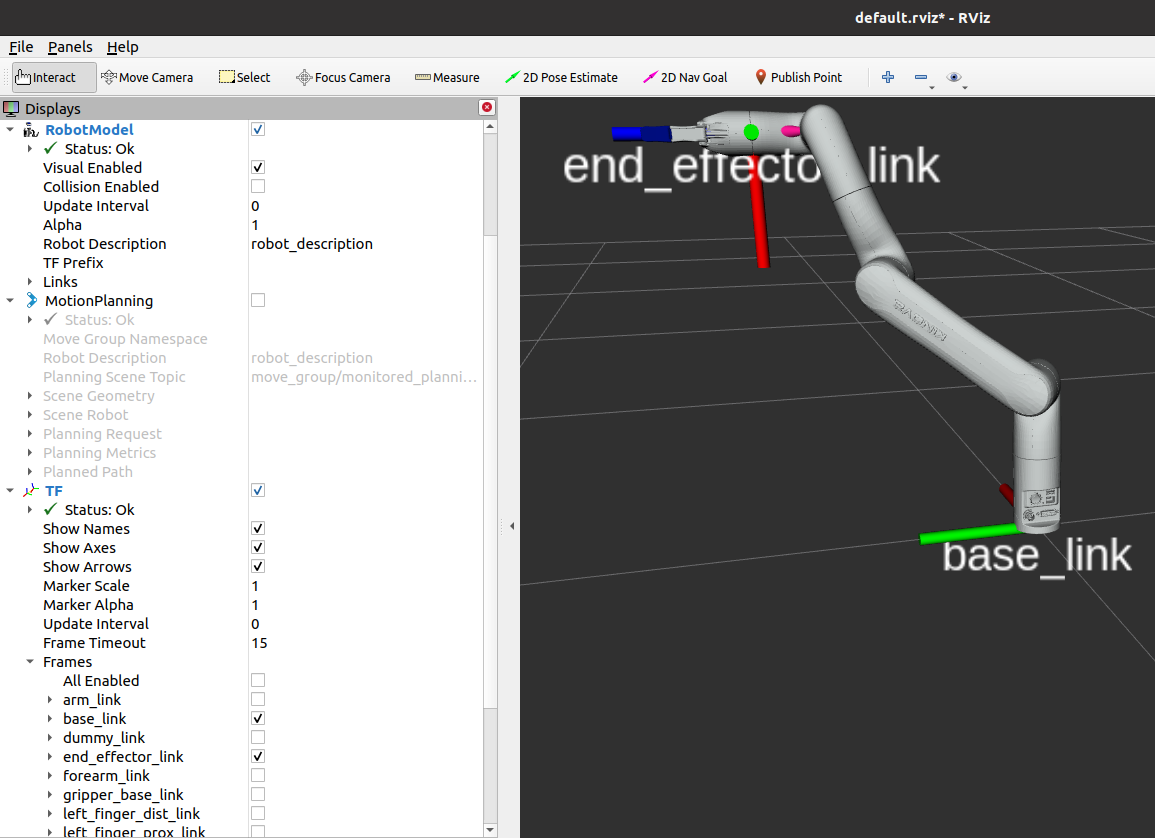
\includegraphics[width=13cm]{images/kinova_rviz.png}\vspace{-4pt}
        \caption{RViZ with Kinova.}\label{fig:kinova_rviz}
        \end{figure}

    \item Use rqt\_tf\_tree to determine the kinematic chain between the two reference frames (base\_link and end\_effector\_link).
    
    \textbf{Answer: }According to the flowchart shown in \mintinline{bash}{rqt_tf_tree}, the kinematic chain between \mintinline{bash}{base_link} and \mintinline{bash}{end_effector_link} can be represented as:

    \textit{$\text{world} \rightarrow \text{base\_link} \rightarrow \text{shoulder\_link} \rightarrow \text{arm\_link} \rightarrow \text{forearm\_link} \rightarrow \text{lower\_wrist\_link} \rightarrow \text{upper\_wrist\_link} \rightarrow \text{end\_effector\_link} \rightarrow \text{dummy\_link}$}
    
    \item Turn on the Motion Planning component again. The "Goal State" in the MotionPlanning panel allows you to set goals to some predefined positions. Inspect it and report what are the reported robot’s joints values and pose of the end effector (wrt the world) when you send the gen3lite to the following preset positions:\\
    
        \begin{enumerate}

            \item Home
            
            \begin{table}[H]
                \caption{Pose information of end effector in home state}
                \begin{subtable}{.5\linewidth}
                    \centering
                    \caption{Position}
                    \begin{tabular}{cccc}
                        \toprule
                        \textbf{Linear} & \textit{x} & \textit{y} & \textit{z} \\\midrule
                        \textbf{Position} & 0.37 & 0.08 & 0.45 \\\bottomrule
                    \end{tabular}
                \end{subtable}
                \begin{subtable}{.5\linewidth}
                    \centering
                    \caption{Orientation}
                    \begin{tabular}{ccccc}
                        \toprule
                        \textbf{Angular} & \textit{x} & \textit{y} & \textit{z} & \textit{w} \\\midrule
                        \textbf{Orientation} & -0.35 & 0.62 & 0.36 & 0.61 \\\bottomrule
                    \end{tabular}
                \end{subtable}
            \end{table}
                    
            \begin{table}[H]
                \centering
                \caption{Joint angles of end effector in home state}
                \begin{tabular}{ccccccc}
                \toprule
                \textbf{Joint} & \textit{1} & \textit{2} & \textit{3} & \textit{4} & \textit{5} & \textit{6} \\\midrule
                \textbf{Angle} & 0 & -16 & 75 & 0 & -60 & 0 \\\bottomrule
                \end{tabular}
            \end{table}

            \item Retract
            
            \begin{table}[H]
                \caption{Pose information of end effector in retract state}
                \begin{subtable}{.5\linewidth}
                    \centering
                    \caption{Position}
                    \begin{tabular}{cccc}
                        \toprule
                        \textbf{Linear} & \textit{x} & \textit{y} & \textit{z} \\\midrule
                        \textbf{Position} & 0.13 & -0.07 & 0.27 \\\bottomrule
                    \end{tabular}
                \end{subtable}
                \begin{subtable}{.5\linewidth}
                    \centering
                    \caption{Orientation}
                    \begin{tabular}{ccccc}
                        \toprule
                        \textbf{Angular} & \textit{x} & \textit{y} & \textit{z} & \textit{w} \\\midrule
                        \textbf{Orientation} & 0.99 & -0.06 & 0.14 & -0.01 \\\bottomrule
                    \end{tabular}
                \end{subtable}
            \end{table}
                    
            \begin{table}[H]
                \centering
                \caption{Joint angles of end effector in retract state}
                \begin{tabular}{ccccccc}
                \toprule
                \textbf{Joint} & \textit{1} & \textit{2} & \textit{3} & \textit{4} & \textit{5} & \textit{6} \\\midrule
                \textbf{Angle} & -3 & 21 & 145 & -88 & -40 & -87 \\\bottomrule
                \end{tabular}
            \end{table}

            \item Select a robot pose that you would choose if you had to pick something from the ground. Add a screenshot of the resulting pose of the arm in \textbf{Gazebo}.
            
            \begin{table}[H]
                \caption{Pose information of end effector in pickup state}
                \begin{subtable}{.5\linewidth}
                    \centering
                    \caption{Position}
                    \begin{tabular}{cccc}
                        \toprule
                        \textbf{Linear} & \textit{x} & \textit{y} & \textit{z} \\\midrule
                        \textbf{Position} & -0.43 & 0.01 & 0.16 \\\bottomrule
                    \end{tabular}
                \end{subtable}
                \begin{subtable}{.5\linewidth}
                    \centering
                    \caption{Orientation}
                    \begin{tabular}{ccccc}
                        \toprule
                        \textbf{Angular} & \textit{x} & \textit{y} & \textit{z} & \textit{w} \\\midrule
                        \textbf{Orientation} & 1.00 & -0.06 & 0.00 & 0.02 \\\bottomrule
                    \end{tabular}
                \end{subtable}
            \end{table}
            
            \begin{table}[H]
                \centering
                \caption{Joint angles of end effector in pickup state}
                \begin{tabular}{ccccccc}
                \toprule
                \textbf{Joint} & \textit{1} & \textit{2} & \textit{3} & \textit{4} & \textit{5} & \textit{6} \\\midrule
                \textbf{Angle} & 5 & 54 & -72 & 93 & -54 & 101 \\\bottomrule
                \end{tabular}
            \end{table}

            \begin{figure}[H]
                \centering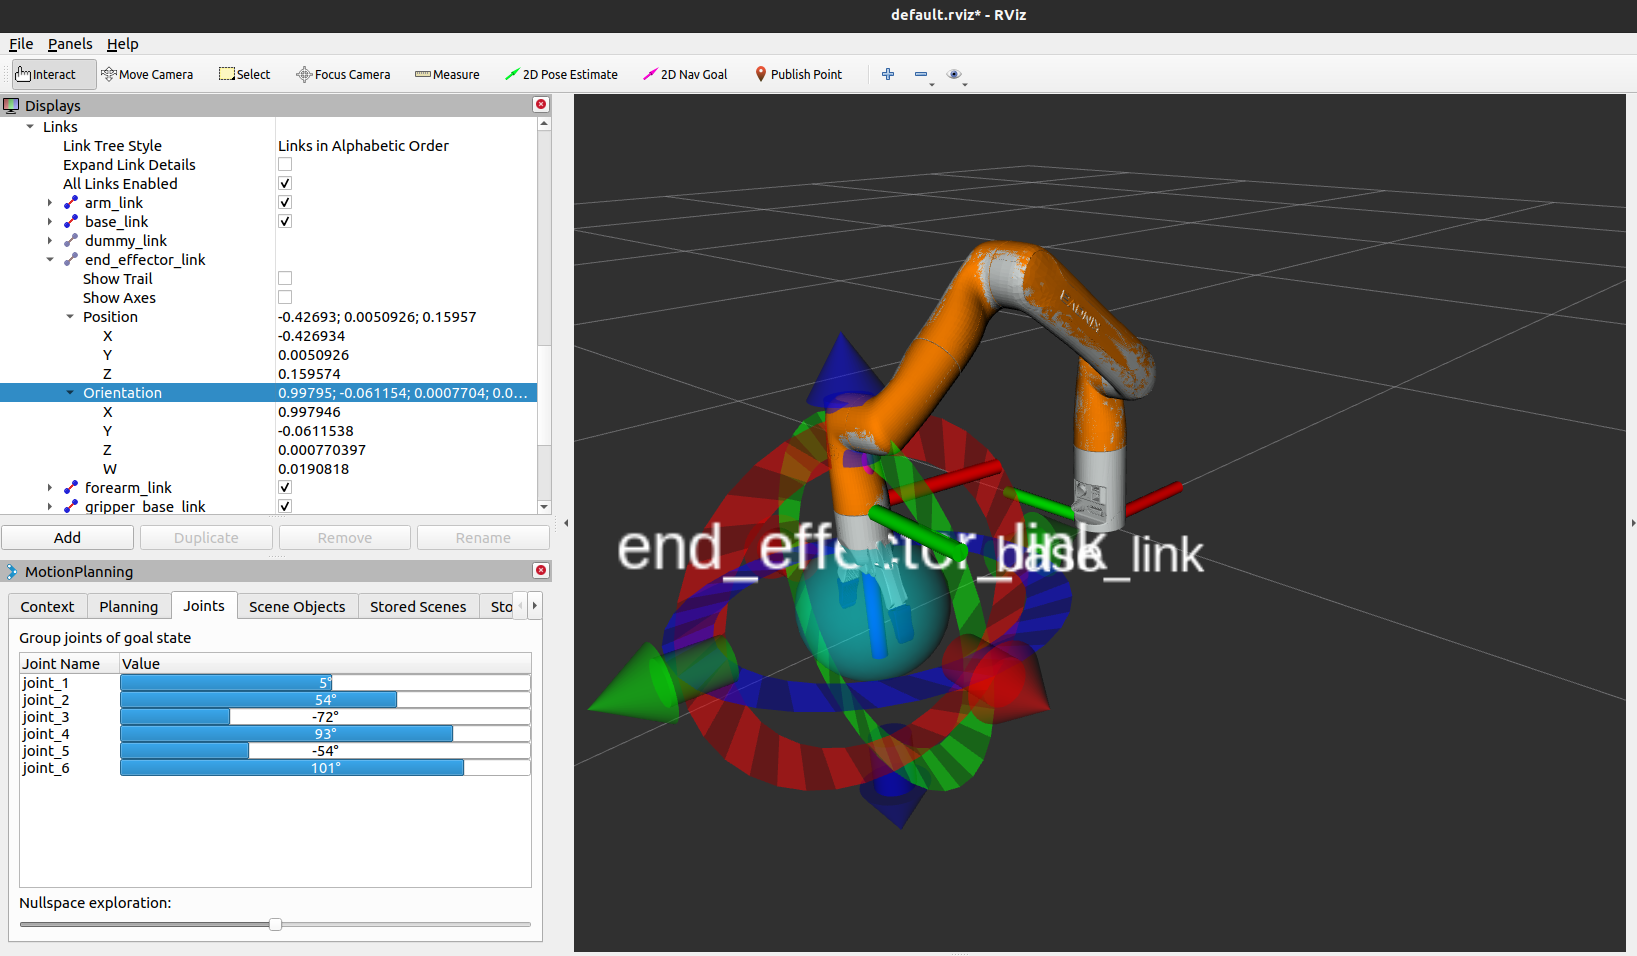
\includegraphics[width=15cm]{images/kinova_pickup.png}
                \caption{Picking up state in RViz from ground with Kinova arm.}\label{fig:kinova_pickup}
            \end{figure}

        \end{enumerate}

\end{enumerate}

\subsection{Using the Joints tab in MotionPlanning to change the robot’s pose on the configuration-space}

In the MotionPlanning panel, find the "Joints" tab. You will be able to change the values of the different joint angles. Explore the configuration space, determine which joints move in which direction when a positive or a negative angle is given to each joint.
\\

\textbf{Deliverables:}

\begin{enumerate}

    \item Configure the joint angles and move to your desired position. Add a screenshot of the rviz window(including joint values and the robot visualization), use the same tools described in the previous subsection to explore the values for the pose and the joint angles.
    
    \begin{table}[H]
        \caption{Pose information of end effector in custom state}
        \begin{subtable}{.4\linewidth}
            \centering
            \caption{Position}
            \begin{tabular}{cccc}
                \toprule
                \textbf{Linear} & \textit{x} & \textit{y} & \textit{z} \\\midrule
                \textbf{Position} & 0.22 & 0.00 & 0.18 \\\bottomrule
            \end{tabular}
        \end{subtable}
        \hfill
        \begin{subtable}{.52\linewidth}
            \centering
            \caption{Orientation}
            \begin{tabular}{ccccc}
                \toprule
                \textbf{Angular} & \textit{x} & \textit{y} & \textit{z} & \textit{w} \\\midrule
                \textbf{Orientation} & 1.00 & -0.02 & 0.04 & -0.01 \\\bottomrule
            \end{tabular}
        \end{subtable}
    \end{table}
    \vspace{-10pt}
    \begin{table}[H]
        \centering
        \caption{Joint angles of end effector in custom state}
        \begin{tabular}{ccccccc}
        \toprule
        \textbf{Joint} & \textit{1} & \textit{2} & \textit{3} & \textit{4} & \textit{5} & \textit{6} \\\midrule
        \textbf{Radian} & 0.30 & -0.35 & 2.34 & -1.57 & -0.38 & -1.22 \\
        \textbf{Degree} & 17 & -20 & 134 & -90 & -22 & -70 \\\bottomrule
        \end{tabular}
    \end{table}

    \begin{figure}[h]
        \centering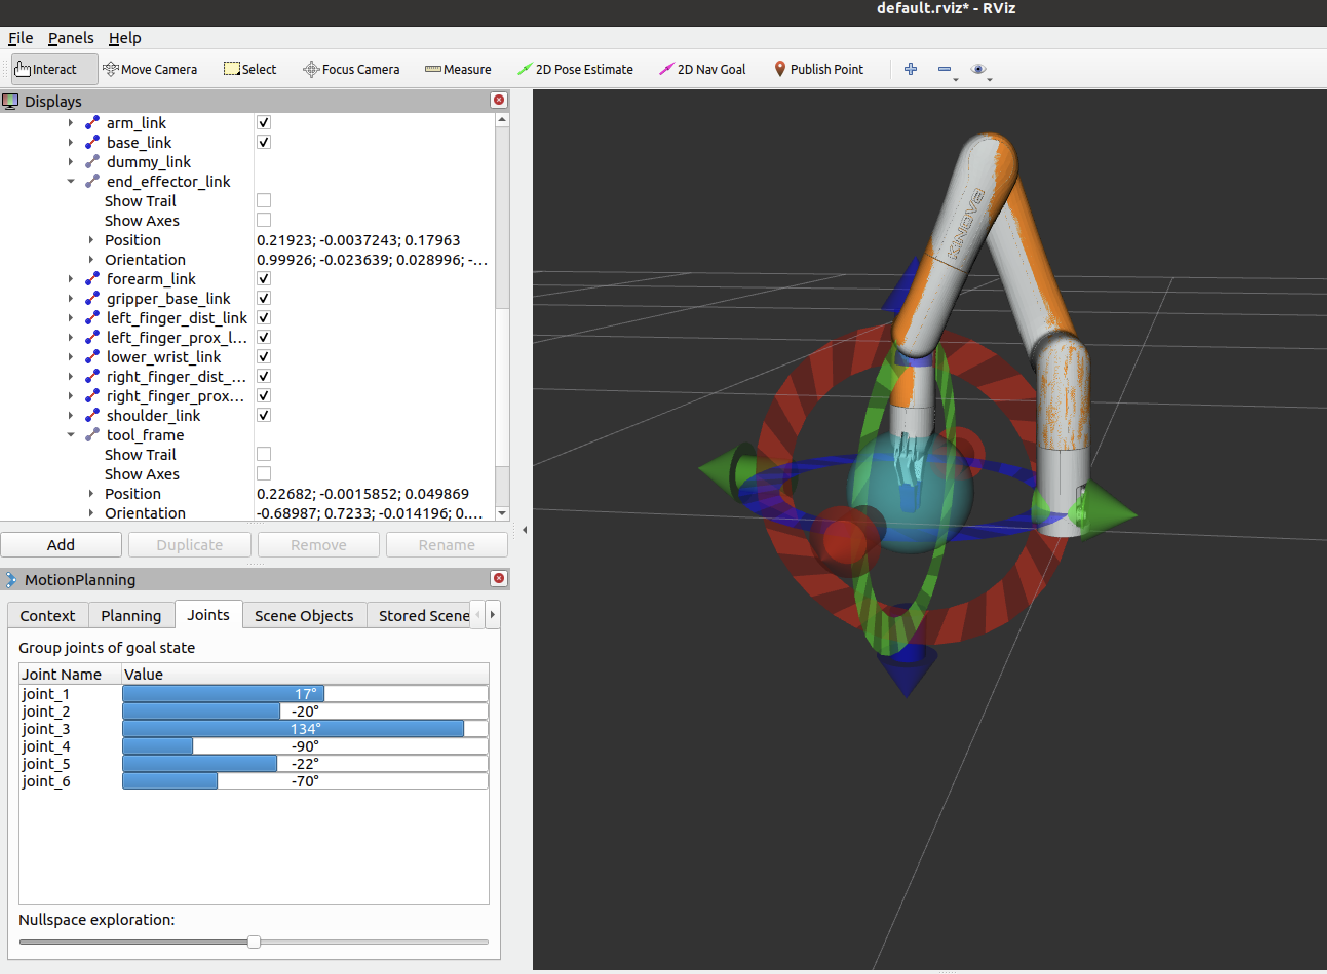
\includegraphics[width=12cm]{images/kinova_custom.png}
        \caption{Custom state of Kinova arm in RViz.}\label{fig:kinova_custom}
    \end{figure}
    
    \item Explain the differences you observed when controlling the robot’s position using either the interactive markers or the joint angles.
    
    \textbf{Answer: }When controlling with the interactive marker, the entire arm moves together, whereas adjusting the angle in the Joint tab moves each corresponding joint.
    \\Serving as the controller for the robot's end effector, the interactive marker changes its positions and orientations, which inevitably requires the synchronized movement of all the joints. This, by definition, is inverse kinematics, the process of which joint parameters are calculated given the end of a kinematic chain.
    \\Changing the position and orientation of each joint from the tab requires less synchronized movement. Upon hitting 'Plan \& Execute' after tuning the angles, the end effector is led to the new position, which is computed with kinematic equations. This, by definition, is forward kinematics.
    
    \item Can you change all joint angles from the RViZ window? If not, explain what degree of freedom is not available and how that impacts the poses you can reach with the robot.
    
    \textbf{Answer: }All the joints can be rotated to almost the full range of degrees for the Kinova arm from the RViz window.    

\end{enumerate}


\section{Introducing Fetch Robot}

\subsection{Fetch Packages Installation}

Following the instructions to install packages from from Fetch Robotics.
\begin{minted}{bash}
    $ cd catkin_ws/src
    $ git clone -b ros1 https://github.com/fetchrobotics/fetch_ros.git
    $ git clone -b gazebo11 https://github.com/fetchrobotics/fetch_gazebo.git
    $ git clone -b ros1 https://github.com/fetchrobotics/fetch_msgs.git
    $ git clone -b ros1 https://github.com/fetchrobotics/power_msgs.git
    $ git clone -b ros1 https://github.com/fetchrobotics/robot_controllers.git
    $ cd ../
    $ rosdep install --from-paths src --ignore-src -y
    (Ignore the error: Unable to locate package ros-noetic-simple-grasping)
    $ sudo apt install ros-noetic-rgbd-launch
\end{minted}
\textbf{Note}:The branch "ros1" and "gazebo11" is developed for ROS Noetic. If you are using other ROS distributions, please git clone to corresponding branch.


\subsection{Fetch Robot Manipulation}
We will go through a similar procedure as the Kinova Gen3lite, familiarizing ourselves with the arm components of the Fetch robot. Execute the following commands in different terminals to spawn a Gazebo simulated Fetch robot, activate the motion capabilities and open an RViZ window

\begin{minted}{bash}
    $ roslaunch fetch_gazebo simulation.launch
    $ roslaunch fetch_moveit_config move_group.launch
    $ rosrun rviz rviz
\end{minted}

You will need to add the Robot Model and the MotionPlanning components in RViZ once it opens. Check the rqt\_tf\_tree to determine the name of the end-effector’s link to run the command:

\begin{minted}{bash}
    $ rosrun tf tf_echo /odom <END-EFFECTOR LINK>
\end{minted}
    
You may also consider using the start of the arm chain as the reference:

\begin{minted}{bash}
    $ rosrun tf tf_echo /<FIRST ARM JOINT> <END-EFFECTOR LINK>
\end{minted}

\begin{figure}[H]
    \vspace{-10pt}
    \centering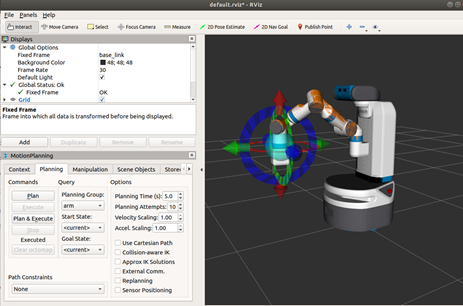
\includegraphics[width=10cm]{images/rviz2.png}
    \caption{Fetch in Rviz.}\label{fig:rviz2}\vspace{-10pt}
    \end{figure}

\textbf{Deliverables:}

\begin{enumerate}

    \item Add a TF component in RViz and enable only the base\_link, the first joint of the arm, and the end\_effector\_link. Disable the Motion Planning component to remove temporarily the interactive markers. Add a screenshot of the RViZ view.

    \begin{figure}[h]
        \centering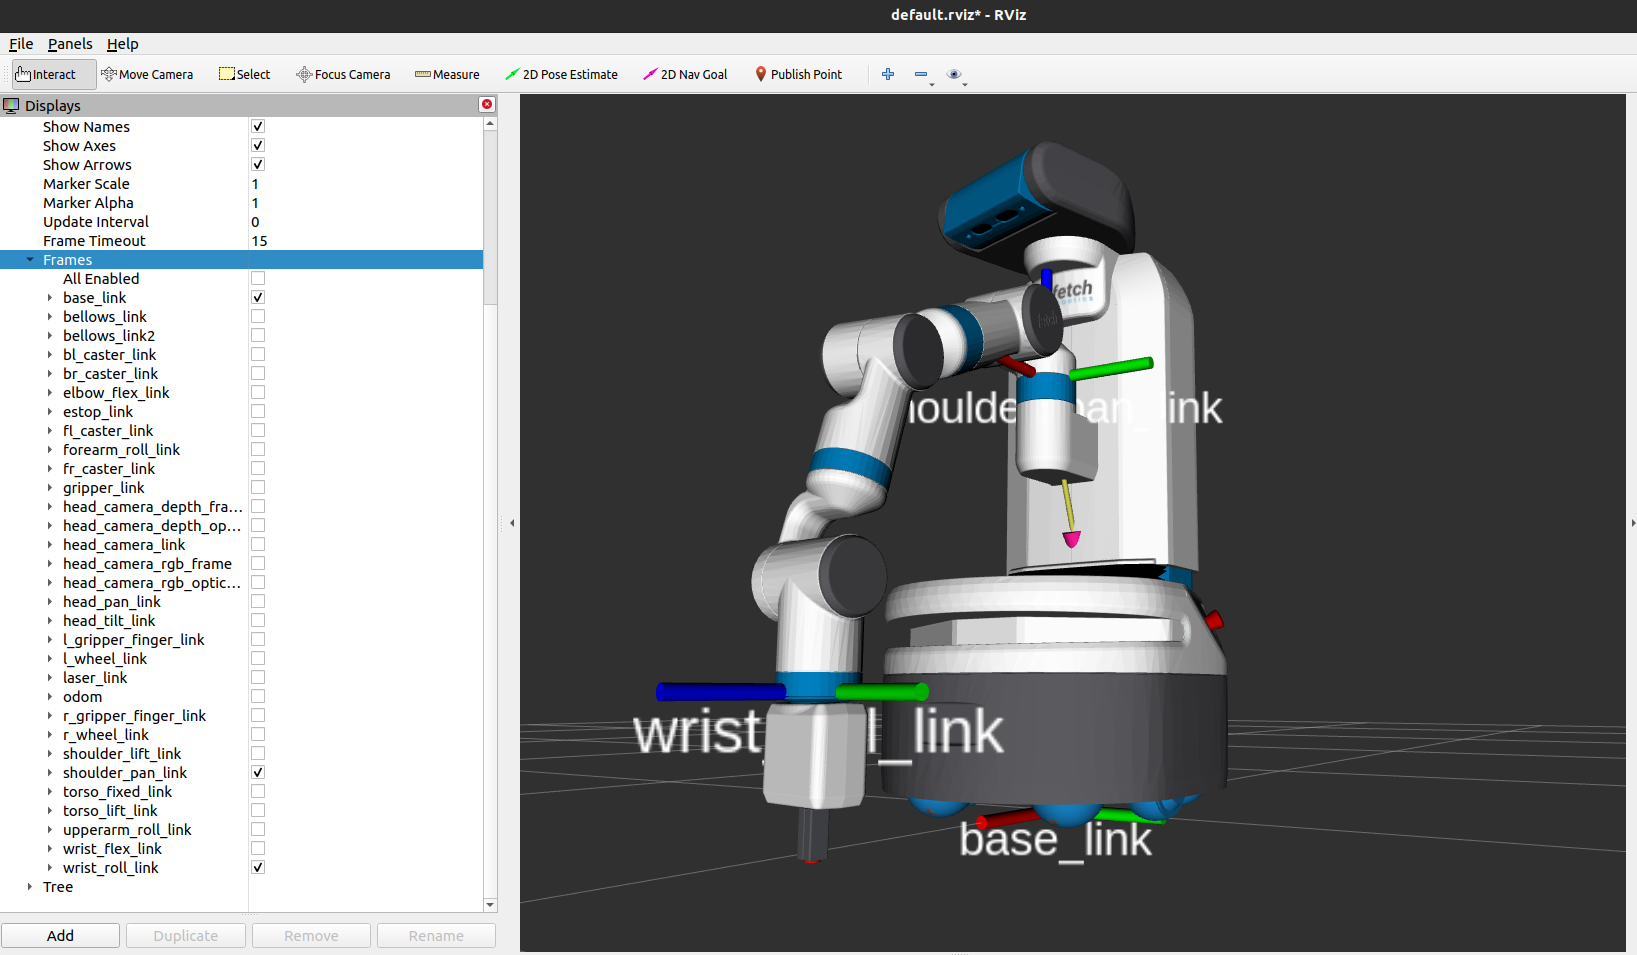
\includegraphics[width=14cm]{images/fetch_default.png}
        \caption{Enabling certain TF components in RViz.}\label{fig:fetch_default}\vspace{-4pt}
    \end{figure}

    \textbf{Answer: }Figure \ref{fig:fetch_default} shows a spawned Fetch robot in RViz with only certain TF components enabled and MotionPlanning disabled. The components requested include links to the base, the first arm joint, and the end effector. Since the definitions of these parts can vary, the following relationships between components and link names are assumed for clarification:

    \begin{minted}{bash}
        <BASE LINK> = base_link
        <FIRST ARM JOINT> = shoulder_pan_link
        <END-EFFECTOR LINK> = wrist_roll_link
    \end{minted}
    \vspace{-10pt}

    \item Use rqt\_tf\_tree to determine the kinematic chain between the two reference frames.
    
    \textbf{Answer: }According to the flowchart shown in \mintinline{bash}{rqt_tf_tree}, the kinematic chain between reference frames, the first joint of arm \mintinline{bash}{shoulder_pan_link} and the end effector \mintinline{bash}{wrist_roll_link}, can be represented as:

    \textit{$\text{base\_link} \rightarrow \text{torso\_lift\_link} \rightarrow \text{shoulder\_pan\_link} \rightarrow \text{shoulder\_lift\_link} \rightarrow \text{upperarm\_roll\_link} \rightarrow \text{elbow\_flex\_link} \rightarrow \text{forearm\_roll\_link} \rightarrow \text{wrist\_flex\_link} \rightarrow \text{wrist\_roll\_link} \rightarrow \text{gripper\_link}$}
    
    \item Unlike the Kinova arm, the MotionPlanning for Fetch does not have preset poses for the arm.
    
    \begin{enumerate}

        \item Show a screenshot of the resulting pose when all joints in the arm are set to 0 degrees.
        
        \begin{figure}[h]
            \centering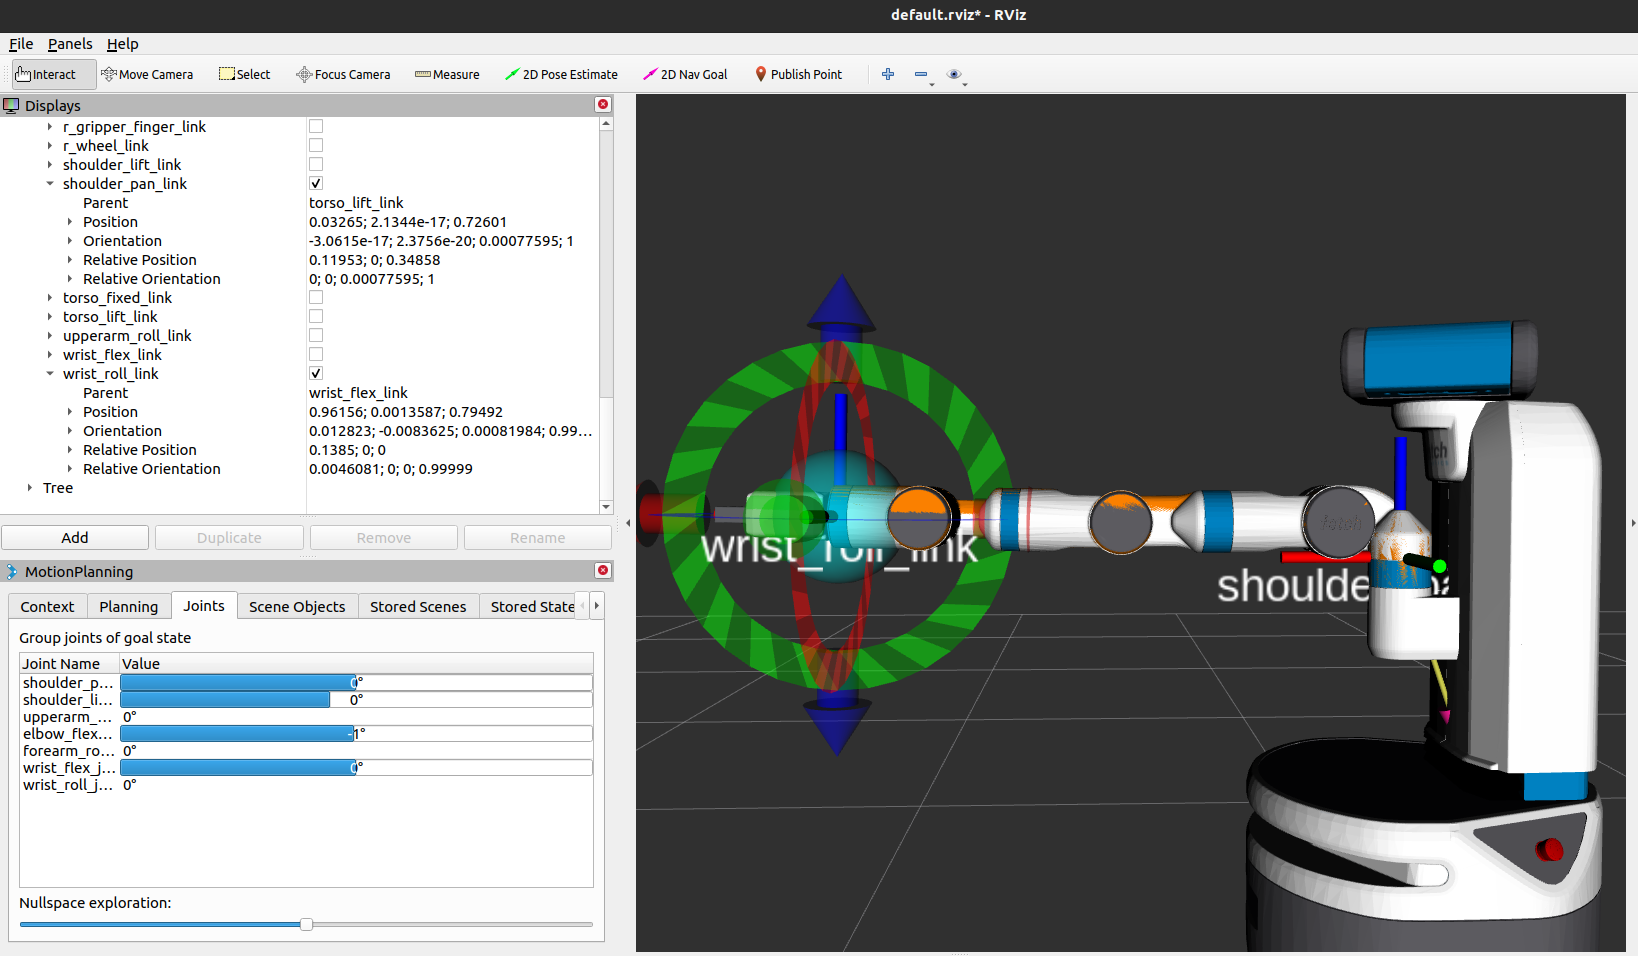
\includegraphics[width=14cm]{images/fetch_zero.png}
            \caption{Setting joint angles to zero.}\label{fig:fetch_zero}\vspace{-4pt}
        \end{figure}

        \textbf{Answer: }Figure \ref{fig:fetch_zero} shows an attempt to set all the joint angles to zero. However, this is the best it can be done. It was found that some joints couldn't be controlled in the Joints tab, while interactive marker couldn't independently control single joints; setting current non-zero angles to zero would also impact on other angles.
        
        \item Report the joint angle values of all Fetch’s arm joints on a pose that would allow Fetch to pick up an object from the floor.
        
        \begin{figure}[h]
            \centering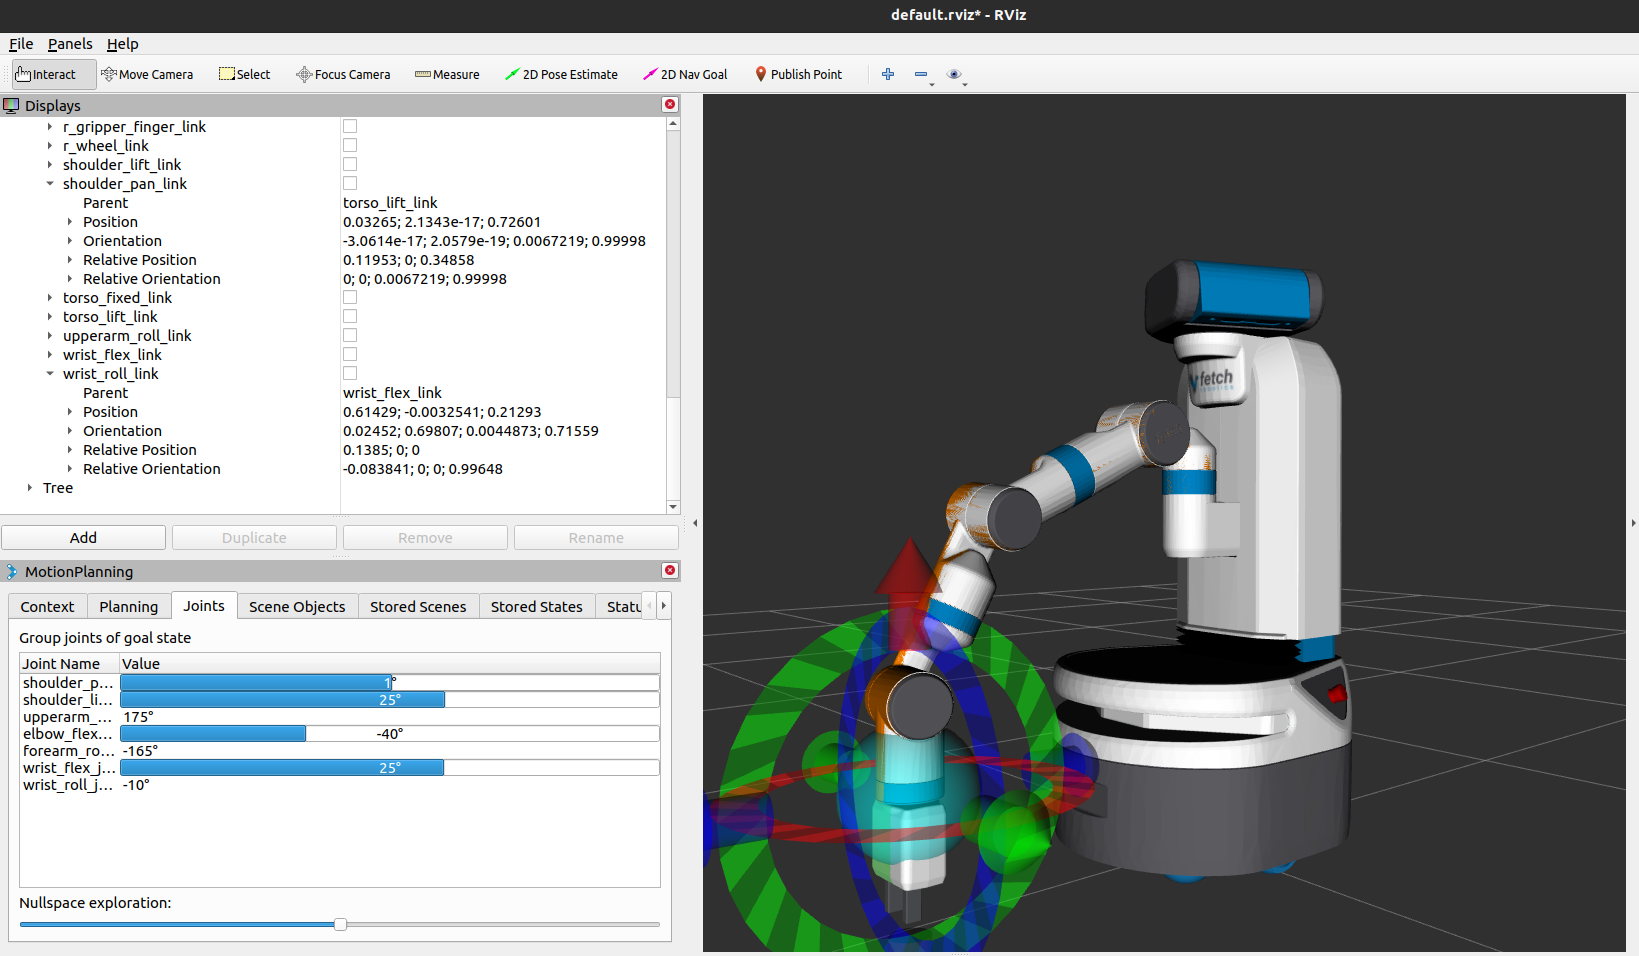
\includegraphics[width=14cm]{images/fetch_pickup.png}
            \caption{Picking up from the ground with Fetch.}\label{fig:fetch_pickup}\vspace{-4pt}
        \end{figure}

        \textbf{Answer: }Figure \ref{fig:fetch_pickup} shows the state, in which the Fetch robot can pick up an object from the ground. The set of joint angle values can be found in the Joint tab.
        
    \end{enumerate}
    
    \item Explain the differences you observed when controlling the robot’s position using either the interactive markers or the joint angles.
    
    \textbf{Answer: }As explained in 2.4.2, controlling with interactive markers is inverse kinematics, and with Joint tab slide bars is forward kinematics. It remains the same that moving the interactive marker will change the angle for all joints, and that most joints can be tuned independently. The difference is that changes to some joint angles can only be made with interactive markers, and will inevitably impact on other joints.
    
    \item Can you change all joint angles from the RViZ window? If not, explain what degree of freedom is not available and how that impacts the poses you can reach with the robot.
    
    \textbf{Answer: }No, not all joint angles can be changed from the Joints tab in RViz.
    \\Among all the joints, \mintinline{bash}{upperarm_roll_link}, \mintinline{bash}{forearm_roll_link} and \mintinline{bash}{wrist_roll_link} can't be tuned with the sliders, but only through interactive markers. That is, none of the roll joints can be controlled in isolation.
    \\For the ones supporting independent manipulation, the degree range of motion is also limited. Unlike the Kinova arm, where the ranges are almost all near $[-180, 180]$, those of the Fetch robot are much more smaller. The joint degree range can be as small as $[-70, 87]$, which belongs to the \mintinline{bash}{shoulder_lift_link}, preventing it from hitting its head. The pattern is that any joint parameter combination that will invite accidental collision with its own torso is prohibited.
    
\end{enumerate}


\section{Using Python to control Fetch robots}

Now that we have familiarized the robot, we will create nodes that will generate motions on Fetch robot. One will move the robot arm by assigning values to joints angle, applying \textbf{forward kinematics} to reach to the target position and orientation of the end-effector in Cartesian space. Another node will apply 
\textbf{inverse kinematics} which calculate and change the joint angles based on the given target pose of the end-effector. You will use working code provided on canvas as a guide. You may need to modify the code to finish the deliverable.

\textbf{Notes:}
You can visit the Fetch documentation for \href{https://docs.fetchrobotics.com/manipulation.html#running-the-pick-and-place-demo}{additional tutorials}.\\

\textbf{Deliverables:}
\begin{enumerate}
    \item Please identify which Python file corresponds to each type of robot kinematics?
    
    \textbf{Answer: }Since joint parameters are computed to move the robot to the goal state, forward kinematics is used in \mintinline{bash}{simple_disco.py}. As the joint angles are calculated based on the pose of the end effector pose, \mintinline{bash}{wave.py} uses inverse kinematics.
    
    \item Capture videos of the robot executing movements using both programs, separately. Upload them to Canvas with your writeup.
    
    \href{https://drive.google.com/file/d/1H86M7AIZrIzaGf10TJZ2XOMb_82X7bvc/view?usp=share_link}{Google Drive link to Fetch robot's simple disco move}
    
    \href{https://drive.google.com/file/d/1LZxnhGoDjbbZgD3olirweqn8HGhDH6gI/view?usp=share_link}{Google Drive link to Fetch robot's wave}
    
    \item Modify the code that performs forward kinematics and move the arm to a pose with your desired input values. Compare the resulting angle values (rostopic echo /joint\_states) to your inputs.

    \begin{table}[H]
        \centering
        \caption{Joint angles of Fetch torso parts in custom state}
        \begin{tabular}{@{}ccccccccc@{}}
        \toprule
        Source & \textit{\begin{tabular}[c]{@{}c@{}}torso\\ lift\end{tabular}} & \textit{\begin{tabular}[c]{@{}c@{}}shoulder\\ pan\end{tabular}} & \textit{\begin{tabular}[c]{@{}c@{}}shoulder\\ lift\end{tabular}} & \textit{\begin{tabular}[c]{@{}c@{}}upperarm\\ roll\end{tabular}} & \textit{\begin{tabular}[c]{@{}c@{}}elbow\\ flex\end{tabular}} & \textit{\begin{tabular}[c]{@{}c@{}}forearm\\ roll\end{tabular}} & \textit{\begin{tabular}[c]{@{}c@{}}  wrist  \\ flex\end{tabular}} & \textit{\begin{tabular}[c]{@{}c@{}}wrist\\ roll\end{tabular}} \\ \midrule
        \mintinline{bash}{simple_disco.py} & 0.00 & 0.65 & -0.77 & 2.15 & -1.17 & 0.73 & -1.40 & -0.77 \\
        \mintinline{bash}{joint_states} & 0.00 & 0.65 & -0.76 & 2.15 & -1.16 & 0.73 & -1.40 & -0.77 \\\bottomrule
        \end{tabular}
    \end{table}

    \textbf{Answer: }The joint parameters reported in \mintinline{bash}{joint_states} highly agree with the ones set in \mintinline{bash}{simple_disco.py}, despite some slight errors.

    \item Modify the code that performs inverse kinematics and move the arm to a pose with your desired input values. Then compare the resulting pose (rosrun tf tf\_echo /<link1> /<link2) to your inputs.
    
    \begin{table}[H]
        \caption{Pose information of end effector in custom state}
        \begin{subtable}{.5\linewidth}
            \centering
            \caption{Position}
            \begin{tabular}{cccc}
                \toprule
                Source & \textit{x} & \textit{y} & \textit{z} \\\midrule
                \mintinline{bash}{wave.py} & 0.042 & 0.384 & 1.826 \\
                \mintinline{bash}{tf_echo} & 0.042 & 0.384 & 1.826 \\\bottomrule
            \end{tabular}
        \end{subtable}
        \hfill
        \begin{subtable}{.5\linewidth}
            \centering
            \caption{Orientation}
            \begin{tabular}{ccccc}
                \toprule
                Source & \textit{x} & \textit{y} & \textit{z} & \textit{w} \\\midrule
                \mintinline{bash}{wave.py} & 0.173 & -0.693 & -0.242 & 0.657 \\
                \mintinline{bash}{tf_echo} & 0.175 & -0.694 & -0.240 & 0.656 \\\bottomrule
            \end{tabular}
        \end{subtable}
    \end{table}

    \textbf{Answer: }The pose information reported in \mintinline{bash}{tf_echo} highly agrees with the one set in \mintinline{bash}{wave.py} as well, despite some slight errors.
    
    \item Discuss what type of robot kinematics was faster to use? Which one was easier to use?
    
    \textbf{Answer: }Forward kinematics is much more efficient in navigating the arm to the goal state, as the only thing required is the ending pose of the end effector. All the joint parameters can be calculated based on this goal, which save a ton of time.
    \\In terms of accuracy and safety, inverse kinematics is the one to pick. Respectively setting each joint angle dictates the shape of the arm and thus prevents accidental collisions. But controlling the arm in RViz is different from terminal, and would yield different results.
    
    \item What were the advantages and disadvantages of using RViz or generated code to control the robot's motion? Please provide at least two thoughts.
    
    \begin{multicols}{2}

        \textsc{RViz}:
        
        \textbf{Pros:}
        \begin{itemize}
            \item easier to navigate
            \item preview goal state
            \item safety warnings
        \end{itemize}
        
        \textbf{Cons:}
        \begin{itemize}
            \item partial joint control
            \item can't set goal pose
        \end{itemize}

    \columnbreak
        \textsc{Code}:
        
        \textbf{Pros:}
        \begin{itemize}
            \item full control over arm
            \item accurate in navigation
            \item easier to deploy
        \end{itemize}
        
        \textbf{Cons:}
        \begin{itemize}
            \item hard to visualize
            \item manual calculations
        \end{itemize}

    \end{multicols}

\end{enumerate}


\end{document}